\documentclass[10pt,a4paper]{article}
\usepackage[utf8]{inputenc} % para poder usar tildes en archivos UTF-8
\usepackage[spanish]{babel} % para que comandos como \today den el resultado en castellano
\usepackage{a4wide} % márgenes un poco más anchos que lo usual
\usepackage{caratula}
% \usepackage[left=3cm,right=3cm,bottom=3cm,top=3cm]{geometry}
%comandos para comentar secciones grandes
\usepackage{comment}
% Comandos para simbolos matematicos.
\usepackage{amsmath, amssymb, tabularx}

% Comandos para referencias
\usepackage{natbib}

% Comandos para Figuras, Graficos, Tikz etc.
\usepackage{tikz}
\usepackage{epsfig}
\usepackage{pgfplots}
\usepackage{graphicx}
\usepackage{epsfig}
\usepackage{caption}
\usepackage{subcaption}
\usepackage{svg}
\usepackage{amssymb}
\usepackage{algorithm}
\usepackage{graphicx}
\usepackage{hyperref}

% Comandos para teoremas etc.
\usepackage{amsthm}
\newtheorem{theorem}{Teorema}
\newtheorem{lemma}[theorem]{Lema}
\newtheorem{proposition}[theorem]{Proposición}
\newtheorem{remark}{Observación}
\newtheorem{corollary}{Corolario}
% \newproof{proof}{Demostración}

% Comandos para algoritmos.
\usepackage[noend]{algpseudocode}
\usepackage{algorithm}
\usepackage{algpseudocode}
\algnewcommand{\IfThenElse}[3]{% \IfThenElse{<if>}{<then>}{<else>}
\State \algorithmicif\ #1\ \algorithmicthen\ #2\ \algorithmicelse\ #3}
\algnewcommand{\IfThen}[2]{% \IfThenElse{<if>}{<then>}
  \State \algorithmicif\ #1\ \algorithmicthen\ #2}
  
  \usepackage{caption}

%\algdef{SE}[SUBALG]{Indent}{EndIndent}{}{\algorithmicend\ }%
%\algtext{Indent}
%\algtext{EndIndent}

\algdef{SE}[SUBALG]{Indent}{EndIndent}{}{\algorithmicend\ }%
\algtext*{Indent}
\algtext*{EndIndent}


%\renewcommand{\baselinestretch}{1.5}

% Comente lo de arriba, porque me parece que es mejor la distancia predeterminada entre renglones. -M

\begin{document}

\titulo{Trabajo práctico: Wiretapping\-}

\fecha{09/2021}

\materia{Teoría de la información}

\integrante{Herrera, Leon}{105/18}{leonazulado@gmail.com}
\integrante{Buceta, Diego}{1/17}{diegobuceta35@gmail.com}
\integrante{Fernández Ortuzar, Agustín}{185/18}{agustinalejofernandezortuzar@gmail.com}


\maketitle

\section{Introducción}
\input{textos/introducción}

\section{Métodos y condiciones de los experimentos}
\section{Métodos y condiciones de los experimentos}

Realizamos capturas de paquetes en distintos horarios en la red LAN hogareña de cada integrante de este trabajo, con el objetivo de obtener un muestreo diverso. Utilizamos la herramienta Wireshark para capturar los paquetes de las redes, que luego exportamos a archivos .csv y .pcap para analizarlos con Pandas. Extendimos el código \texttt{Python} provisto para que tome como fuente un archivo .pcap en lugar de capturar la red en tiempo real, calcule la frecuencia e información de cada símbolo y la entropía de las fuentes y luego escriba los resultados en archivos .csv para estudiarlos.

\begin{table}[H]
    \begin{center}
        \begin{tabular}{||c c c c c c||} 
             \hline
             Dataset & Tecnología & Tamaño de la red & Tamaño de la muestra & Hora & Día \\ [0.5ex] 
             \hline\hline
             $Red 1$ & Wi-Fi & Red LAN & 39511 tramas & 15:20hs & Viernes \\ 
             \hline
             $Red 2$ & Wi-Fi & Red LAN & 23841 tramas & 16hs & Sábado \\
             \hline
             $Red 3$ & Wi-Fi & Red LAN & 50695 tramas & 19:40hs & Viernes \\ [1ex] 
             \hline
        \end{tabular}
    \end{center}
    \caption{Características de las capturas}
    \label{tab: condiciones de datasets}
\end{table}


\subsection{Contexto de las capturas} 

\begin{description}
    \item[Hogar del integrante 1 (dataset \emph{Red1}):] En el momento del análisis, había una computadora y un celular conectados a la red wifi. Se capturaron paquetes durante una hora, haciendo un uso de multimedia sobre la red. Se obtuvieron 39511 tramas. 
    
    \item[Hogar del integrante 2 (dataset \emph{Red2}):] Se capturaron paquetes durante una hora desde una computadora portatil conectada a una red wifi doméstica con acceso a Internet, en la que además se hallaban conectados dos celulares, una tablet, dos cámaras de seguridad y dos televisores. Dentro del transcurso de la captura, se ejecutó una aplicación que determina los dispositivos que están conectados a una red wi-fi y, como se desarrolla más adelante, esto tuvo un efecto en los resultados obtenidos.
    
    \item[Hogar del integrante 3 (dataset \emph{Red3}):] Desde una computadora portatil, se capturaron paquetes durante una hora en una red doméstica. En esta red estaban ademas conectados: Una computadora de escritorio por ethernet, dos celulares y un repetidor de wi-fi al que estaban probablemente conectadas una tablet y una computadora portatil.

\end{description}

\subsection{Explicación del código}
\subsubsection{Análisis 1 - Fuente $S_{1}$}
Tomando como base el código dado por la cátedra, restaba agregar funciones que se encarguen de calcular la frecuencia e información de cada símbolo, la entropía de la fuente y el porcentaje de tráfico \texttt{Broadcast} vs \texttt{Unicast}.

Habiendo procesado los paquetes de cada muestra, obtuvimos un diccionario donde los símbolos eran las claves y el valor era la cantidad de apariciones durante el análisis. Para calcular la frecuencia de cada símbolo iteramos por las claves del diccionario y calculamos su porcentaje de apariciones frente a todos los paquetes.

Para calcular la información de cada símbolo, calculamos el logaritmo base 2 de la frecuencia de cada uno (calculado previamente) y lo negamos.
 
Finalmente, dado que nuestra fuente no es equiprobable, calculamos la \texttt{entropía} como la suma de la multiplicación de la información que provee cada símbolo y su frecuencia.
\begin{equation} \label{eq24}
\begin{split}
H(S) = {\sum_{s \in S}frecuencia_{s} * informacion_{s}}
\end{split}
\end{equation}

Respecto del cálculo del porcentaje de tráficco \texttt{Broadcast} vs \texttt{Unicast}, lo que hicimos fue contar sus apariciones durante el análisis de las muestras.

\subsubsection{Análisis 2 - Fuente $S_{2}$}
Dado que necesitamos distinguir los hosts de paquetes \texttt{ARP} que habían aparecido durante las mediciones de cada muestreo, decidimos utilizar como símbolo la dirección \texttt{IP} origen de la trama. Este valor se encuentra en el atributo \texttt{psrc} de los paquetes \texttt{ARP}. Como se muestra en la Figura~\ref{code: callback_2} tomamos las direcciones \texttt{IP} origen de cada paquete recibido y aumentamos el contador correspondiente en el diccionario S2 obteniendo al finalizar la cantidad total de apariciones de cada una.

Los calculos de la información y frecuencia por símbolo, así como también entropía se hace de forma análoga al análisis 1.

\begin{figure}[H]
    \includegraphics[width=0.7\textwidth]{images/resultados_generales/codigo_analisis_2.png}\vspace{1em}
    \centering
    \caption{Función ejecutada al procesar cada trama de la muestra}
    \label{code: callback_2}
\end{figure}

\subsection{Justificación de elección de la fuente $S_{2}$} 
Como mencionamos previamente, con el objetivo de distinguir hosts de nuestra red definimos como símbolos a las direcciones \texttt{IP} origen de las tramas. Esta elección nos resultó natural debido a que, si un dispositivo se encuentra en una red, es altamente probable que en algún momento envíe un paquete y no solo se dedique a recibir.

Otra opción que tuvimos en cuenta fue tomar como símbolos las direcciones \texttt{IP} destino de las tramas, aunque rápdiamente notamos que podrían aparecer tramas con destinos inexistentes en la red, por lo que no era una opción viable. Luego pudimos comprobar que éste efectivamente era un caso posible: durante el análisis del comportamiento de las redes presentadas en el trabajo, notamos cómo algunas aplicaciones hacian uso de técnicas de fuerza bruta para, por ejemplo, encontrar los hosts activos en la red. Esto generaba muchas tramas donde la dirección \texttt{IP} destino no era un nodo válido dentro de la red.



\newpage
\section{Resultados de los experimentos}
\subsection{Casa integrante 1 - dataset $Red 1$} 

La entropía calculada fue de 0.049668, un valor bajo lo cuál indica que cada símbolo obtenido no arroja mucha información y es predecible.


\begin{figure}[H]\begin{center}
  \includegraphics[width=0.6\textwidth]{images/freq_ws_4_info.png}\vspace{1em}
  \caption{Frecuencias por protocolo}
\end{center}\end{figure}


\texttt{IPV4} (con 0.9955\%) fue el protocolo más escuchado en contraposición contra \texttt{ARP} (0.0019\%) e \texttt{IPV6} (0.0024\%), lo cuál tiene sentido por la naturaleza de estos últimos. Recordemos que ARP es un protocolo utilizado para encontrar la dirección MAC de un host a partir de su \texttt{IP} en la red y actualizar su tabla \texttt{ARP}. Esto sólo es necesario hacerlo cuando la tabla de un host no contiene una entrada para el host con el que quiere comunicarse. Si tenemos en cuenta la baja cantidad de dispositivos en la red es más que razonable obtener una tan baja presencia de \texttt{ARP}.

\begin{figure}[H]
    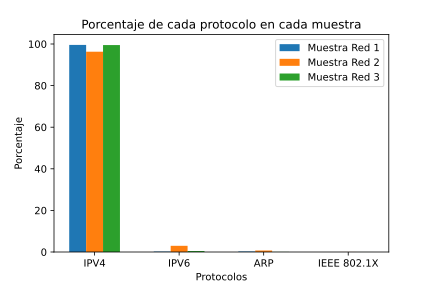
\includegraphics[scale=0.6]{images/resultados_generales/porcentaje_cada_protocolo_cada_muestra.png}\vspace{1em}
    \centering
    \caption{Porcentaje de cada protocolo en cada muestra capturada}
    \label{fig: porcentajes}
\end{figure}

Se pueden observar que el protocolo IPv4 domina las 3 redes, como es de esperarse. La red 2 


\begin{figure}[H]
    \centering
    \begin{subfigure}{0.45\linewidth}
        \includegraphics[scale=0.45]{images/resultados_diego/red_1_info.png}
        \caption{Red 1}
        \label{fig: info red 1}
    \end{subfigure}
    \begin{subfigure}{0.5\linewidth} 
        \includegraphics[scale=0.45]{images/resultados_agus/red_2_info.png}
        \caption{Red 2}
        \label{fig: info red 2}
    \end{subfigure}
    \begin{subfigure}{0.5\linewidth} 
        \centering
        \includegraphics[scale=0.45]{images/resultados_lion/red_3_info.png}
        \caption{Red 3}
        \label{fig: info red 3}
    \end{subfigure}
    \caption{Cantidad de información por cada símbolo en cada muestra.}
    \label{fig: informacion de los simbolos}
\end{figure}



Dado que la entropía es muy baja, la aparición de símbolos como \texttt{ARP} e \texttt{IPV6} aportan mucha información dada su escasa aparición.
\begin{figure}[H]
    \centering
    \begin{subfigure}[b]{0.3\textwidth}
        \centering
        \includegraphics[width=\textwidth]{images/resultados_diego/red_1_broadcast_unicast.png}
        \caption{Red 1}
        \label{fig: b/u red 1}
    \end{subfigure}
    \begin{subfigure}[b]{0.3\textwidth} 
        \centering
        \includegraphics[scale=0.7, width=\textwidth]{images/resultados_agus/red_2_broadcast_unicast.png}
        \caption{Red 2}
        \label{fig: b/u red 2}
    \end{subfigure}
    \begin{subfigure}[b]{0.3\textwidth} 
        \centering
        \includegraphics[width=\textwidth]{images/resultados_lion/red_3_broadcast_unicast.png}
        \caption{Red 3}
        \label{fig: b/u red 3}
    \end{subfigure}
    \caption{Proporción de Broadcast/Unicast en cada muestra.}
    \label{fig: informacion de los simbolos}
\end{figure}

\begin{table}[H]\begin{center}
  \begin{tabular}{|c|c|}
  \hline
  \textbf{Tráfico} & \textbf{Frecuencia} \\ \hline
  \texttt{Unicast   }&  0.998\%     \\ \hline
  \texttt{Broadcast      }&  0.0014\%     \\ \hline
  \end{tabular}
  \caption{Frecuencia de Unicast y Broadcast en la $Red 1$}
  \label{Red 1}
\end{center}\end{table}

\begin{table}[H]\begin{center}
  \begin{tabular}{|c|c|}
  \hline
  \textbf{Tráfico} & \textbf{Frecuencia} \\ \hline
  \texttt{Unicast   }&  0.9682\%     \\ \hline
  \texttt{Broadcast      }&  0.0317\%     \\ \hline
  \end{tabular}
  \caption{Frecuencia de Unicast y Broadcast en la $Red 2$}
  \label{Red 2}
\end{center}\end{table}

\begin{table}[H]\begin{center}
  \begin{tabular}{|c|c|}
  \hline
  \textbf{Tráfico} & \textbf{Frecuencia} \\ \hline
  \texttt{Unicast   }&  0.9862\%     \\ \hline
  \texttt{Broadcast      }&  0.0037\%     \\ \hline
  \end{tabular}
  \caption{Frecuencia de Unicast y Broadcast en la $Red 3$}
  \label{Red 3}
\end{center}\end{table}


La diferencia de porcentajes entre uno se debe a que \texttt{BROADCAST} es el tipo de tráfico de los paquetes ARP que por lo anterior vimos tienen bajas apariciones, mientras que UNICAST representa mayoritariamente todo el otro tráfico, por ejemplo, el que ocurrió durante el consumo de multimedia, que también por lo anterior, vimos eran los paquetes con mayor aparición.


\subsection{Casa integrante 2 - dataset $Red 2$}

• Porcentaje de tráfico Broadcast/Unicast sobre el tráfico total.

 - Broadcast: 756
 - Unicast: 23085


• Porcentaje de aparición de cada protocolo encontrado.

 - IPV4: 0.9629
 - ARP: 0.0297
 - IPV6: 0.0071
 - 34958: 0.0003
 
• Entropía de la red: 0.2572

• Cantidad de información de cada símbolo comparado con la entropía de la red.

 - IPV4: 0.0546
 - ARP: 5.0715
 - IPV6: 7.1318
 - 34958: 11.9562

\begin{table}[H]
\begin{center}
    \begin{tabular}{||c c||} 
        \hline
        Dataset & Entropía \\ [0.5ex] 
        \hline\hline
        $Red 1$ & $0.04966814662839276$ \\ 
        \hline
        $Red 2$ & $0.3494232951207893$ \\
        \hline
        $Red 3$ & $0.08226822373062319$ \\ [1ex] 
        \hline
    \end{tabular}
    \caption{Tabla de Entropía en las redes}
    \label{Tabla entropía}
\end{center}
\end{table}


\subsection{Fuente de información $S_{2}$ - Hosts distinguidos en la red } 
\subsubsection{Casa integrante 1 - dataset $Red 1$}

\begin{figure}[H]
    \centering
    \begin{subfigure}{0.5\linewidth} 
        \includegraphics[scale=0.5]{images/resultados_generales/red_1_info.png}
        \centering
        \caption{Red 1}
    \end{subfigure}
    \begin{subfigure}{0.5\linewidth} 
        \includegraphics[scale=0.5]{images/resultados_generales/red_2_info.png}
        \centering
        \caption{Red 2}
    \end{subfigure}
    \begin{subfigure}{0.5\linewidth} 
        \centering
        \includegraphics[scale=0.45]{images/resultados_generales/red_3_info.png}
        \caption{Red 3}
    \end{subfigure}
    \caption{Cantidad de información por cada símbolo en cada muestra.}
    \label{fig: informacion de los simbolos}
\end{figure}

\newpage
\section{Conclusión}
\section{Conclusión}


\textbf{¿Considera que las muestras obtenidas analizadas son representativas del comportamiento general de la red?} %Esto puede quedarse en esta sección%

\begin{description}
    \item[Red 1]: Es representativa. Había pocos dispositivos conectados y el uso se mantuvo constante a lo largo de toda la medición lo cuál resulto en una gran predominancia \texttt{IPv4} (mayormente con UDP como protocolo en el nivel superior) y pocos \texttt{ARP}, ya que no se conectaban nuevos dispositivos ni cambiaba la comunicación.
    
    \item[Red 2]: No es representativo porque se utilizó una aplicación que revisa qué dispositivos están conectados en la red wifi, y para ello emitió una gran cantidad de broadcasts consultando por las direcciones IP dentro de un rango.

    \item[Red 3]: Es representativo, ya que el uso que se le estaba dando a la red era el habitual en nuestra vivienda. Subida y bajada constante de datos es habitual por la profesión de los integrantes de esta red.
        
\end{description}

A excepción de unas pocas sorpresas, los resultados cayeron dentro de lo que esperabamos. Es clara la predominancia del protocolo \texttt{IPV4} en las tramas de cada red escuchada. Esto en parte es razonable, debido a la naturaleza de \texttt{ARP} (sólo es necesario cuando no se tiene una dirección MAC, una vez obtenida no se vuelve a solicitar con mucha frecuencia) y la baja adopción que tiene actualmente \texttt{IPv6}, aunque en el futuro cercano se volverá imprescindible. 


\newpage

\textbf{¿Hay alguna relación entre la entropía de las redes y alguna característica de las mismas (ej.:tamaño, tecnología, etc)?} %Esto tambien puede quedarse

Notamos que obtuvimos mediciones muy similares para las 3 redes y en base al análisis creemos que se debe justamente a las características que comparten: topologías (tipo estrella), usos (al menos durante la escucha) y tecnología (Wi-Fi).










\end{document}
